% !TeX program = xelatex
% !TeX encoding = UTF-8

%%%%%%%%%%%%%%%%%%%%%%%%%%%%%%%%%%%%%%%%%%%%%%%%%%%%%%%%%%%%%%%
%
% 文档信息
% File:      main.tex
% Author:    R W
% Email:     no.thanks@example.com
% Date:      2025/06/02
% Version:   v0.0.1
% Log:       Initial version
%
% 内容描述:
% 本文档为西安理工大学学士学位论文的LaTeX模板
% 
%
% 注意事项:
% 1. 编译方式使用XeLaTeX
% 2. 文章中的插图存放在figures下, 支持pdf, png, jpg, jpeg等格式
% 3. 其他文件: 引用文献列表文件reference.bib, 引用文献格式模板xaut.bst, 文章排版格式模板xautthsis.sty
% 4. 若使用的是本地编译器, 则直接双击word_count.cmd文件, 或者在Powershell中使用word_count.ps1即可查看总字数和各小节字数
%%%%%%%%%%%%%%%%%%%%%%%%%%%%%%%%%%%%%%%%%%%%%%%%%%%%%%%%%%%%%%%

\documentclass[UTF8, twoside]{ctexart}
\usepackage{mathtools, wallpaper}

% 编码 & 字体配置
\usepackage[T1]{fontenc}
\usepackage{pagecolor}
\usepackage{lmodern}
\usepackage{microtype}

% 数学 & 图表
\usepackage{cite}  % 用于引用
\usepackage{hyperref}  % 用于引用跳转
\usepackage{caption}  % 用于修改图标名称
\usepackage{subfigure}  % 可以添加子图
\usepackage{amssymb}  % mathbb字体
\usepackage{amsmath}
\usepackage{indentfirst}  % 首行缩进
\usepackage{ulem}  % 在导言区添加, 提供 \uline
\usepackage{etoolbox} % patch 命令
\normalem

\usepackage{xautthesis}  % 自定义格式

\begin{document}
\captionsetup[figure]{labelfont={bf},name={图},labelsep=space}

\thispagestyle{empty}
% 封面居中排版
\begin{center}
    \vspace*{3.3cm}

    {\lishu\fontsize{52}{52}\selectfont 毕业设计(论文)}

    \vspace{3.5cm}

    {\fontsize{17}{17}\selectfont
        \begin{tabular}{@{}lc@{}}
            \makebox[4em][s]{题目}   & \uline{\makebox[12em][s]{\hfill 这里填写题目 \hfill}}   \\[0.55em]
                                   & \uline{\makebox[12em][s]{\hfill 这里填写题目 \hfill}}   \\[0.55em]
            \makebox[4em][s]{专业}   & \uline{\makebox[12em][s]{\hfill ******** \hfill}} \\[0.55em]
            \makebox[4em][s]{班级}   & \uline{\makebox[12em][s]{\hfill ******** \hfill}} \\[0.55em]
            \makebox[4em][s]{学生}   & \uline{\makebox[12em][s]{\hfill ******** \hfill}} \\[0.55em]
            \makebox[4em][s]{指导教师} & \uline{\makebox[12em][s]{\hfill ******** \hfill}}
        \end{tabular}
    }

    \vfill

    
\includegraphics{logo/logo.png}

    \vspace{1cm}

    {\fontsize{17}{17}\selectfont \underline{\hspace{4em} ******** \hspace{4em}} 年}

\end{center}
\newpage

% 中文摘要
\pagenumbering{Roman}

\begingroup
\centering % 居中
\heiti\bfseries % 应用 Arial 字体, 加粗
\fontsize{16}{18}\selectfont % 三号字(14pt)
\parbox{0.8\textwidth}{\centering
    这里填写题目
}\par
\endgroup

\titlespacing*{\section}{0pt}{0pt}{0pt}
\vspace*{0.6cm}
\section*{摘\quad 要}
\markboth{摘要}{}
\vspace*{0.2cm}
随着时代的发展,计算机视觉这一学科成为计算机科学研究中的热门领域,视觉跟踪是计算机视觉的核心领域之一。这一技术越来越多的应用在视频监控系统,解放人力的同时提升系统工作效率,以便及时应对一些突发情况。
本文在视频监控的基础上,展开对运动目标检测以及运动目标跟踪这两个问题的学习与研究。本文的主要工作包括分析、比较了帧差法、平均法建立背景模型、单高斯背景建模和混合高斯背景建模法(使用多个高斯分布描述像素点的背景与前景像素,并利用线性逼近来更新背景模型来完成对运动目标的提取)这几种运动目标检测算法。学习了基于粒子滤波算法(通过给运动目标分配一个粒子集群来模拟估计运动目标的具体位置,并且对粒子集群进行更新保证能对运动目标的有效跟踪)的视频运动目标跟踪。
本文在Visual Studio 2015编译器上用C++程序语言、OpenCV视觉库,实现了混合高斯背景建模的方法来提取运动目标,粒子滤波算法来跟踪运动目标。在不同场景下对视频中人、汽车等运动目标测试取得良好的效果。

\vspace{1.4em}
\noindent\textbf{关键词}: 背景减除; 粒子滤波; 背景建模; 高斯分布
\newpage

% 英文摘要
\pagenumbering{Roman}

\newfontfamily{\arialfont}{Arial} % 定义临时字体命令
\begingroup
\centering % 居中
\arialfont\bfseries % 应用 Arial 字体, 加粗
\fontsize{14}{16}\selectfont % 四号字(14pt), 行距 16pt
\parbox{0.8\textwidth}{\centering
    Fill in the title of the thesis here
}\par
\endgroup

\vspace*{1cm}
\section*{\arialfont\bfseries Abstract}
\titlespacing*{\section}{0pt}{0pt}{34pt}
\markboth{\arialfont Abstract}{}
\vspace*{0.2cm}
With the development of the times, the field of computer vision has become a hot field in computer science research. Visual tracking is one of the core areas of computer vision. This technology is more and more applications in the video surveillance system, the liberation of human resources at the same time enhance the efficiency of the system in order to deal with some unexpected situations in a timely manner.
On the basis of video surveillance, this paper starts the study and research on the two problems of moving target detection and moving target tracking. The main work of this paper includes the analysis of the frame difference method, the average method to establish the background model, single Gaussian background modeling and mixed Gaussian background modeling method (using multiple Gaussian distributions to describe the background and foreground pixels of the pixel, and using linear approximation To update the background model to complete the extraction of moving objects) these several motion target detection algorithm. The video moving target tracking based on the particle filter algorithm (by allocating a particle cluster to the moving object to simulate the specific position of the moving target and updating the particle cluster to ensure the effective tracking of the moving target) is studied.
In this paper, a hybrid Gaussian background modeling method is used to extract moving objects and particle filter algorithms to track moving objects in C ++ program language and OpenCV visual library in Visual Studio 2015 compiler. In different scenes on the video of people, cars and other sports target test to achieve good results.

\vspace{1.4em}
\noindent\textbf{Key words}: background subtraction; particle filter ;background modeling; gaussian distributiontraining
\newpage

% 目录
\pagenumbering{Roman}
\tableofcontents
\newpage

\pagenumbering{arabic}
\vspace*{3pt}
\section{绪论}
\subsection{选题背景和意义}
深度学习是一种机器学习方法, 它通过构建多层神经网络来自动学习数据中的特征表示\cite{LeCun2015}。与传统方法相比, 深度学习能从原始数据中提取更复杂、高层次的特征, 特别适用于图像识别、语音识别、自然语言处理等任务\cite{alexnet, hinton2012deep}。其核心在于通过大量数据和计算, 逐层优化网络参数, 实现从输入到输出的端到端建模\cite{LeCun2015}。

\subsection{国内外研究现状}
目前,国际上许多高校和研究所,如麻省理工学学院等都专门设立了专门针对运动目标检测的研究组或者研究实验室。美英等国家已经跟进了大量的相关项目。一些著名公司和研究机构、知名院校,如IBM、微软、麻省理工学院等都投入了大量的人力物力来进行智能监控系统的研究,有一些成果已经转化为产品投入了市场。
目前在国内的研究机构中,中国科学院北京自动化研究所下属的模式识别国家重点实验室视觉监控研究处于领先地位。国内其他高校如上海交通大学等也对这方面进行了研究。国内一些企业也对计算机视觉有所涉猎,如海康威视等。同时国内一些核心期刊也刊登了一批计算机视觉的研究成果。

\subsection{研究内容}
本文主要研究内容是......

\subsection{论文组织结构}
目前在国内的研究机构中,中国科学院北京自动化研究所下属的模式识别国家重点实验室视觉监控研究处于领先地位。国内其他高校如上海交通大学等也对这方面进行了研究。国内一些企业也对计算机视觉有所涉猎,如海康威视等。同时国内一些核心期刊也刊登了一批计算机视觉的研究成果。

目前在国内的研究机构中,中国科学院北京自动化研究所下属的模式识别国家重点实验室视觉监控研究处于领先地位。国内其他高校如上海交通大学等也对这方面进行了研究。国内一些企业也对计算机视觉有所涉猎,如海康威视等。同时国内一些核心期刊也刊登了一批计算机视觉的研究成果。

本文整体划分为五个章节。具体组织编排如下所示:

第一章为绪论, 主要介绍了本篇毕业设计的选题背景和意义, 在国内外的研究和发展状况, 主要研究内容以及文章总体组织结构。

第二章为基础知识介绍, 主要讲解了......

第三章为......

第四章为实验设计, 介绍了......

第五章为总结, 对本文的工作进行了总结, 并在展望中提出了模型的问题和改进方向。

\vspace*{3pt}
\cleardoublepage
\section{基础知识介绍}
\subsection{卷积神经网络}
引用示例\cite{lenet1998,alexnet}。插入公式示例, 如公式\eqref{cnn_fun}:
\begin{align}
    (I * K)_{i, j}=\sum_m \sum_n I(i + m, j + n) \cdot K(m, n) + b
    \label{cnn_fun}
\end{align}

插入单张图像示例, 插入图片示例, 如图\ref{cnn_fig}所示。
\begin{figure}[tbhp]
    \centering
    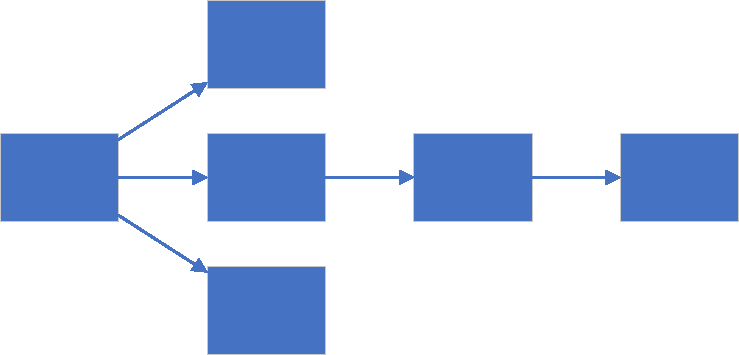
\includegraphics[scale=0.5]{figures/1.pdf}
    \caption{图片标题}
    \label{cnn_fig}
\end{figure}

插入多图示例, 图\ref{act_fun}。
\begin{figure}[tbhp]
    \centering
    \subfigure[子图标题]
    {
        \begin{minipage}[b]{.3\linewidth}
            \centering
            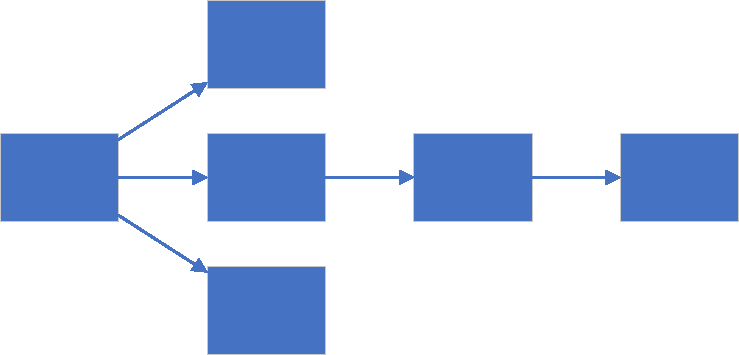
\includegraphics[scale=0.3]{figures/1.pdf}
        \end{minipage}
    }
    \subfigure[子图标题]
    {
        \begin{minipage}[b]{.3\linewidth}
            \centering
            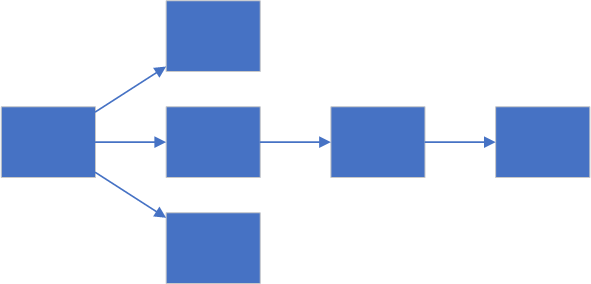
\includegraphics[scale=0.3]{figures/1.png}
        \end{minipage}
    }
    \subfigure[子图标题]
    {
        \begin{minipage}[b]{.3\linewidth}
            \centering
            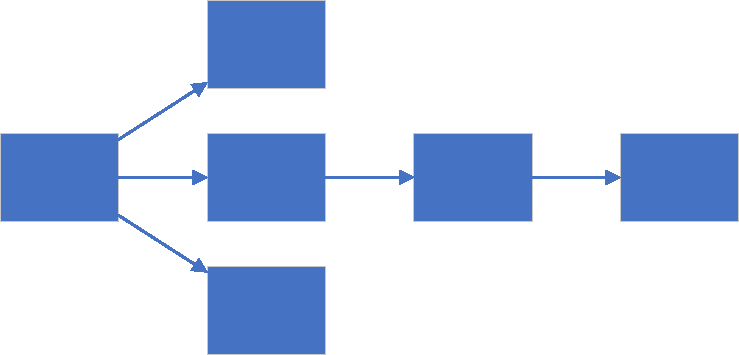
\includegraphics[scale=0.3]{figures/1.pdf}
        \end{minipage}
    }
    \caption{图片标题}
    \label{act_fun}
\end{figure}

\subsubsection{前向传播}
CNN前向传播

\subsubsection{反向传播}
CNN反向传播

\subsection{本章小结}
这里是本章小结



\vspace*{3pt}
\cleardoublepage
\section{第三章标题}
\subsection{引言}
...

\subsection{总体流程设计}
...




\vspace*{3pt}
\cleardoublepage
\section{实验设计}
结果如表\ref{tab:FLOP}所示。
\begin{table}[tbhp]
    \centering
    \caption{表格标题}
    \label{tab:FLOP}
    \begin{tabular}{ccccc}
        \hline
        描述 & ... & ... & ... & ... \\
        \hline
        描述 & ... & ... & ... & ... \\
        描述 & ... & ... & ... & ... \\
        描述 & ... & ... & ... & ... \\
        描述 & ... & ... & ... & ... \\
        \hline
    \end{tabular}
\end{table}




\vspace*{3pt}
\cleardoublepage
\section{总结与展望}
\subsection{总结}
...

\subsection{展望}
...



\cleardoublepage
\section*{致谢}
\markboth{致谢}{}
\addcontentsline{toc}{section}{致谢}
...



\cleardoublepage
\addcontentsline{toc}{section}{参考文献}
\bibliographystyle{xaut}
\bibliography{reference}

\end{document}
